%
% 6.006 problem set 2
%
\documentclass[12pt,twoside]{article}

\input{../macros}

\usepackage{amsmath}
\usepackage{url}
\usepackage{mdwlist}
\usepackage{graphicx}
\usepackage{clrscode3e}
\usepackage{listings}
\usepackage{tikz}
\usetikzlibrary{arrows}
\usetikzlibrary{matrix}
\usetikzlibrary{positioning}
\usetikzlibrary{shapes.geometric}
\usetikzlibrary{shapes.misc}
\usetikzlibrary{trees}

\setlength{\oddsidemargin}{0pt}
\setlength{\evensidemargin}{0pt}
\setlength{\textwidth}{6.5in}
\setlength{\topmargin}{0in}
\setlength{\textheight}{8.5in}

% Fill these in!
\newcommand{\theproblemsetnum}{2}
\newcommand{\releasedate}{September 15, 2011}
\newcommand{\partaduedate}{Tuesday, September 27}
\newcommand{\tabUnit}{3ex}
\newcommand{\tabT}{\hspace*{\tabUnit}}

\begin{document}

\handout{Problem Set \theproblemsetnum}{\releasedate}

\newcommand{\solution}[1]{
  \par\medskip
  \textbf{Solution:} #1
}
% \renewcommand{\solution}[1]{ }

\textbf{Both theory and programming questions} are due {\bf \partaduedate} at
{\bf 11:59PM}.
%
Please download the .zip archive for this problem set, and refer to the
\texttt{README.txt} file for instructions on preparing your solutions.

Remember, your goal is to communicate. Full credit will be given only
to a correct solution which is described clearly. Convoluted and
obtuse descriptions might receive low marks, even when they are
correct. Also, aim for concise solutions, as it will save you time
spent on write-ups, and also help you conceptualize the key idea of
the problem.

We will provide the solutions to the problem set 10 hours after the problem set
is due, which you will use to find any errors in the proof that you submitted.
You will need to submit a critique of your solutions by \textbf{Thursday,
September 29th, 11:59PM}. Your grade will be based on both your solutions and
your critique of the solutions.

\medskip

\hrulefill

\begin{problems}

\problem \points{40} \textbf{Fractal Rendering}

You landed a consulting gig with Gopple, who is about to introduce a new line
of mobile phones with Retina HD displays, which are based on unicorn e-ink and thus
have infinite resolution. The high-level executives heard that fractals have
infinite levels of detail, and decreed that the new phones' background will be
the  \defn{Koch snowflake} (Figure \ref{fig:snowflake}).

\begin{figure}[htbp]
\centering
\includegraphics[width=0.4\textwidth]{figures/snowflake.pdf}
\caption{The Koch snowflake fractal, rendered at Level of Detail (LoD) 0 through 5.}
\label{fig:snowflake}
\end{figure}

Unfortunately, the phone's processor (CPU) and the graphics chip (GPU) powering
the display do not have infinite processing power, so the Koch fractal cannot be
rendered in infinite detail. Gopple engineers will stop the recursion at a
fixed depth $n$ in order to cap the processing requirement. 
For example, at $n=0$, the fractal is just a triangle.
Because higher depths result in more detailed drawing, this depth is usually
called the \defn{Level of Detail (LoD)}.

The Koch snowflake at LoD $n$ can be drawn using an algorithm following the
sketch below:

\begin{codebox} 
\Procname{$\proc{Snowflake}(n)$}
\li $e_1, e_2, e_3 \gets
\textrm{edges of an equilateral triangle with side length }1$
\li $\proc{Snowflake-Edge}(e_1, n)$
\li $\proc{Snowflake-Edge}(e_2, n)$
\li $\proc{Snowflake-Edge}(e_3, n)$
\end{codebox}

\begin{codebox}
\Procname{$\proc{Snowflake-Edge}(\id{edge}, n)$}
\li \If $n \isequal 0$
\li   \Then \textrm{\id{edge} is an edge on the snowflake}
\li \Else
\li   $e_1, e_2, e_3 \gets \textrm{split \id{edge} in 3 equal parts}$
\li   $\proc{Snowflake-Edge}(e_1, n - 1)$
\li   $f_2, g_2 \gets \textrm{edges of an equilateral triangle whose 3rd edge
is } e_2 \textrm{, pointing outside the snowflake}$
\li   $\textrm{$\Delta(f_2,g_2,e_2)$ is a triangle on the snowflake's surface}$
\li   $\proc{Snowflake-Edge}(f_2, n - 1)$
\li   $\proc{Snowflake-Edge}(g_2, n - 1)$
\li   $\proc{Snowflake-Edge}(e_3, n - 1)$
    \End
\end{codebox}

The sketch above should be sufficient for solving this problem. If you are
curious about the missing details, you may download and unpack the problem set's
\texttt{.zip} archive, and read the CoffeeScript implementation in
\texttt{fractal/src/fractal.coffee}.

In this problem, you will explore the computational requirements of four
different methods for rendering the fractal, as a function of the LoD~$n$.
For the purpose of the analysis, consider the recursive calls to
\proc{Snowflake-Edge}; do not count the main call to \proc{Snowflake} as part
of the recursion tree.
(You can think of it as a super-root node at a special level -1, but it behaves 
differently from all other levels, so we do not include it in the tree.) Thus,
the recursion tree is actually a forest of trees, though we still refer to the
entire forest as the ``recursion tree''. The root calls to \proc{Snowflake-Edge}
are all at level~$0$.

Gopple's engineers have prepared a prototype of the Koch fractal drawing
software, which you can use to gain a better understanding of the problem. To
use the prototype, download and unpack the problem set's \texttt{.zip} archive,
and use Google Chrome to open \texttt{fractal/bin/fractal.html}.

%We will use $n$ to name the fixed depth at which the recursion is halted. For
%example, at $n=0$ the fractal is a triangle. 

%\begin{problemparts}

%\problempart
First, in 3D hardware-accelerated rendering (e.g., iPhone), surfaces are
broken down into triangles (Figure \ref{fig:snowflake-triangle}). The CPU
compiles a list of coordinates for the triangles' vertices, and the GPU
is responsible for producing the final image. So, from the CPU's
perspective, rendering a triangle costs the same, no matter what its surface
area is, and the time for rendering the snowflake fractal is proportional to the
number of triangles in its decomposition.

\begin{figure}[htbp]
\begin{center}
\includegraphics[width=0.2\textwidth]{figures/snowflake-triangle.pdf}
\end{center}
\caption{Koch snowflake drawn with triangles.}
\label{fig:snowflake-triangle}
\end{figure}

\begin{problemparts}
  \problempart \points{1} What is the height of the recursion tree for rendering
  a snowflake of LoD $n$?
    \begin{enumerate}
      \item $\log n$
      \item $n$
      \item $3 \, n$
      \item $4 \, n$
    \end{enumerate}
  \solution {
    At level 0, the argument to \proc{Snowflake-Edge} is $n$. At each level in
    the recursion tree, the argument decreases by $1$. At level $n$, the
    argument to \proc{Snowflake-Edge} becomes 0, which triggers the termination
    condition at the beginning of the function. See the figure below.
    
    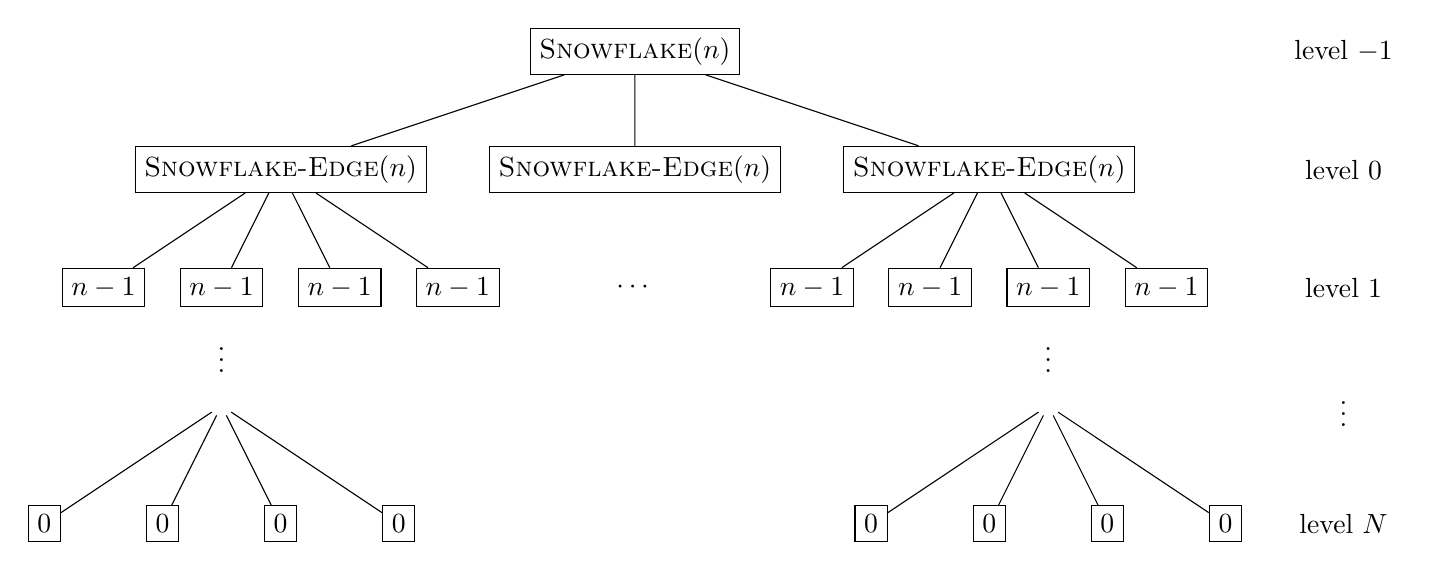
\begin{tikzpicture}
      [level 1/.style={sibling distance=45mm},
      level 2/.style={sibling distance=15mm}]
    \node [rectangle, draw] {$\proc{Snowflake}(n)$}
    child {
      node [rectangle, draw] {$\proc{Snowflake-Edge}(n)$}
      child {
        node [rectangle, draw] {$n - 1$}
      }
      child {
        node [rectangle, draw] {$n - 1$}
        child {
          node {}
          child {
            node [rectangle, draw] {$0$}
          }
          child {
            node [rectangle, draw] {$0$}
          }
          child {
            node [rectangle, draw] {$0$}
          }
          child {
            node [rectangle, draw] {$0$}
          }
          edge from parent[draw=none] node {$\vdots$}
        }
      }
      child {
        node [rectangle, draw] {$n - 1$}
      }
      child {
        node [rectangle, draw] {$n - 1$}
      }
    }
    child {
      node [rectangle, draw] {$\proc{Snowflake-Edge}(n)$}
      child {
        node {$\cdots$} edge from parent[draw=none] 
      }
    }
    child {
      node [rectangle, draw] {$\proc{Snowflake-Edge}(n)$}
      child {
        node [rectangle, draw] {$n - 1$}
      }
      child {
        node [rectangle, draw] {$n - 1$}
      }
      child {
        node [rectangle, draw] {$n - 1$}
        child {
          node {}
          child {
            node [rectangle, draw] {$0$}
          }
          child {
            node [rectangle, draw] {$0$}
          }
          child {
            node [rectangle, draw] {$0$}
          }
          child {
            node [rectangle, draw] {$0$}
            child [grow=right] {
              node {level $N$} edge from parent[draw=none]
              child [grow=up] {
                node {$\vdots$} edge from parent[draw=none]
                child [grow=up] {
                  node {level $1$} edge from parent[draw=none]
                  child [grow=up] {
                    node {level $0$} edge from parent[draw=none]
                    child [grow=up] {
                      node {level $-1$} edge from parent[draw=none]
                    }
                  }
                }
              }
            }
          }
          edge from parent[draw=none] node {$\vdots$}
        }
      }
      child {
        node [rectangle, draw] {$n - 1$}
      }
    };
    \end{tikzpicture}
  }
  \problempart \points{2} How many nodes are there in the recursion tree at
  level $i$, for $0 \le i \le n$?
    \begin{enumerate}
      \item $3 ^ i$
      \item $4 ^ i$
      \item $4 ^ {i + 1}$
      \item $3 \cdot 4 ^ i$
    \end{enumerate}
  \solution {
    \proc{Snowflake} calls \proc{Snowflake-Edge} once for each side of the
    initial triangle, so there are 3 nodes at level 0. At levels $0 \le i <
    n$, \proc{Snowflake-Edge} makes 4 calls to itself, so each node at those
    levels has 4 children. This works out to $3 \cdot 4 ^ i$ nodes at level $i$.
  }
  \problempart \points{1} What is the asymptotic rendering time (triangle count)
  for a node in the recursion tree at level $i$, for $0 \le i < n$?
    \begin{enumerate}
      \item $0$
      \item $\Theta(1)$
      \item $\Theta(\frac{1}{9}^i)$
      \item $\Theta(\frac{1}{3}^i)$
    \end{enumerate}
  \solution {
    Levels 0 through $n - 1$ draw one triangle (spike) for each side that is
    split into 4 line segments. So the cost is always $\Theta(1)$ / node.
  }
  \problempart \points{1} What is the asymptotic rendering time (triangle count)
  at each level $i$ of the recursion tree, for $0 \le i < n$?
    \begin{enumerate}
      \item 0
      \item $\Theta(\frac{4}{9} ^ i)$
      \item $\Theta(3 ^ i)$
      \item $\Theta(4 ^ i)$
    \end{enumerate}
  \solution{
    $\Theta(4 ^ i)$, obtained by multiplying the previous two
    answers and reducing the result to the simplest form.
  }
  \problempart \points{2} What is the total asymptotic cost for the CPU, when
  rendering a snowflake with LoD $n$ using 3D hardware-accelerated rendering?
    \begin{enumerate}
      \item $\Theta(1)$
      \item $\Theta(n)$
      \item $\Theta(\frac{4}{3}^n)$
      \item $\Theta(4^n)$
    \end{enumerate}
  \solution{
    At level $n$ (\proc{Snowflake-Edge} has argument 0), the termination
    condition is triggered, and no triangle is drawn.
    Summing up over all the other levels of the recursion tree, we obtain $$T(n)
    = \sum_{i=0}^{n - 1}{\Theta(4^i)} = \Theta(4^n)$$
    
    The recursion for one side of the snowflake can be written as
    \[
    T(n)=\left\{\begin{array}{ll}
         \Theta(1), &\text{if } n = 0, \\
         4T(n-1)+\Theta(1), &\text{if } n \ge 1.
         \end{array}\right. 
    \]
  }
\end{problemparts}

%\problempart
Second, when using 2D hardware-accelerated rendering, the surfaces'
outlines are broken down into open or closed paths (list of connected
line segments). For example, our snowflake is one closed path composed of
straight lines. The CPU compiles the list of cooordinates in each path to be
drawn, and sends it to the GPU, which renders the final image. This approach is
also used for talking to high-end toys such as laser cutters and plotters.

\begin{problemparts}
  \problempart \points{1} What is the height of the recursion tree for rendering
  a snowflake of LoD $n$ using 2D hardware-accelerated rendering?
    \begin{enumerate}
      \item $\log n$
      \item $n$
      \item $3 \, n$
      \item $4 \, n$
    \end{enumerate}
  \solution {
    $n$, because the recursion tree is the same as in the previous part.
  }
  \problempart \points{1} How many nodes are there in the recursion tree at
  level $i$, for $0 \le i \le n$?
    \begin{enumerate}
      \item $3 ^ i$
      \item $4 ^ i$
      \item $4 ^ {i + 1}$
      \item $3 \cdot 4 ^ i$
    \end{enumerate}
  \solution {
    $3 \cdot 4 ^ i$, because the recursion tree is the same as in the previous
    part.
  }
  \problempart \points{1} What is the asymptotic rendering time (line segment
  count) for a node in the recursion tree at level $i$, for $0 \le i < n$?
    \begin{enumerate}
      \item $0$
      \item $\Theta(1)$
      \item $\Theta(\frac{1}{9}^i)$
      \item $\Theta(\frac{1}{3}^i)$
    \end{enumerate}
  \solution {
    Line segments are only rendered at the last level, so the cost is 0 for
    levels $0 \le i < n$.
  }
  \problempart \points{1} What is the asymptotic rendering time (line segment
  count) for a node in the last level $n$ of the recursion tree?
    \begin{enumerate}
      \item $0$
      \item $\Theta(1)$
      \item $\Theta(\frac{1}{9}^n)$
      \item $\Theta(\frac{1}{3}^n)$
    \end{enumerate}
  \solution {
    At the last level, each side is turned into one straight line, so the cost
    is $\Theta(1)$ / node.
  }
  \problempart \points{1} What is the asymptotic rendering time (line segment
  count) at each level $i$ of the recursion tree, for $0 \le i < n$?
    \begin{enumerate}
      \item 0
      \item $\Theta(\frac{4}{9} ^ i)$
      \item $\Theta(3 ^ i)$
      \item $\Theta(4 ^ i)$
    \end{enumerate}
  \solution{
    0, because all the line segments are rendered at the last level.
  }
  \problempart \points{1} What is the asymptotic rendering time (line segment
  count) at the last level $n$ in the recursion tree?
    \begin{enumerate}
      \item $\Theta(1)$
      \item $\Theta(n)$
      \item $\Theta(\frac{4}{3}^n)$
      \item $\Theta(4^n)$
    \end{enumerate}
  \solution{
    We multiply two previous answers and reduce the result to the simplest form:
    $$3 \cdot 4 ^ n \cdot \Theta(1) = \Theta(4^n).$$
  }
  \problempart \points{1} What is the total asymptotic cost for the CPU, when
  rendering a snowflake with LoD $n$ using 2D hardware-accelerated rendering?
    \begin{enumerate}
      \item $\Theta(1)$
      \item $\Theta(n)$
      \item $\Theta(\frac{4}{3}^n)$
      \item $\Theta(4^n)$
    \end{enumerate}
  \solution{
    The sum of the previous two answers: $T(n) = \Theta(4^n)$.
  }
\end{problemparts}

%\problempart
Third, in 2D rendering without a hardware accelerator (also called
software rendering), the CPU compiles a list of line segments for each path like
in the previous part, but then it is also responsible for ``rasterizing'' each
line segment. Rasterizing takes the coordinates of the segment's endpoints and
computes the coordinates of all the pixels that lie on the line segment.
Changing the colors of these pixels effectively draws the line segment on the
display. We know an algorithm to rasterize a line segment in time proportional
to the length of the segment. It is easy to see that this algorithm is optimal,
because the number of pixels on the segment is proportional to the segment's
length. Throughout this problem, assume that all line segments have length
at least one pixel, so that the cost of rasterizing is greater than the cost
of compiling the line segments.

It might be interesting to note that the cost of 2D software rendering is
proportional to the total length of the path, which is also the power required
to cut the path with a laser cutter, or the amount of ink needed to print the
path on paper.

\begin{problemparts}
  \problempart \points{1} What is the height of the recursion tree for rendering
  a snowflake of LoD $n$?
    \begin{enumerate}
      \item $\log n$
      \item $n$
      \item $3 \, n$
      \item $4 \, n$
    \end{enumerate}
  \solution {
    $n$, because the recursion tree is the same as in the previous part.
  }
  \problempart \points{1} How many nodes are there in the recursion tree at
  level $i$, for $0 \le i \le n$?
    \begin{enumerate}
      \item $3 ^ i$
      \item $4 ^ i$
      \item $4 ^ {i + 1}$
      \item $3 \cdot 4 ^ i$
    \end{enumerate}
  \solution {
    $3 \cdot 4 ^ i$, because the recursion tree is the same as in the previous
    part.
  }
  \problempart \points{1} What is the asymptotic rendering time (line segment
  length) for a node in the recursion tree at level $i$, for $0 \le i < n$?
  Assume that the sides of the initial triangle have length 1.
    \begin{enumerate}
      \item $0$
      \item $\Theta(1)$
      \item $\Theta(\frac{1}{9}^i)$
      \item $\Theta(\frac{1}{3}^i)$
    \end{enumerate}
  \solution {
    Line segments are only rendered at the last level, so the cost is 0 for
    levels $0 \le i < n$
  }
  \problempart \points{1} What is the asymptotic rendering time (line segment
  length) for a node in the last level $n$ of the recursion tree?
    \begin{enumerate}
      \item $0$
      \item $\Theta(1)$
      \item $\Theta(\frac{1}{9}^n)$
      \item $\Theta(\frac{1}{3}^n)$
    \end{enumerate}
  \solution {
    At level 0, each side has length 1. Levels 0 through $n - 1$ split a
    length-$l$ side into 4 length-$\frac{l}{3}$ segments. So, at each level $0
    \le i \le n$, the length of a side is $\frac{1}{3}^i$. Specifically, at
    level $n$, each segment has length $\frac{1}{3}^n = \Theta(\frac{1}{3}^n)$.
  }
  \problempart \points{1} What is the asymptotic rendering time (line segment
  length) at each level $i$ of the recursion tree, for $0 \le i < n$?
    \begin{enumerate}
      \item 0
      \item $\Theta(\frac{4}{9} ^ i)$
      \item $\Theta(3 ^ i)$
      \item $\Theta(4 ^ i)$
    \end{enumerate}
  \solution{
    0, because all the line segments are rendered at the last level.
  }
  \problempart \points{1} What is the asymptotic rendering time (line segment
  length) at the last level $n$ in the recursion tree?
    \begin{enumerate}
      \item $\Theta(1)$
      \item $\Theta(n)$
      \item $\Theta(\frac{4}{3}^n)$
      \item $\Theta(4^n)$
    \end{enumerate}
  \solution{
    We multiply two previous answers and reduce the result to the simplest form.
    $$3 \cdot 4 ^ n \cdot \Theta(\frac{1}{3}^n) =
    \Theta(\frac{4}{3}^n)$$ }
  \problempart \points{1} What is the total asymptotic cost for the CPU, when rendering
  a snowflake with LoD $n$ using 2D software (not hardware-accelerated)
  rendering?
   \begin{enumerate}
      \item $\Theta(1)$
      \item $\Theta(n)$
      \item $\Theta(\frac{4}{3}^n)$
      \item $\Theta(4^n)$
    \end{enumerate}
  \solution{
    The sum of the previous two answers. $T(n) = \Theta(\frac{4}{3}^n)$
  }
\end{problemparts}

%\problempart
The fourth and last case we consider is 3D rendering without hardware
acceleration. In this case, the CPU compiles a list of triangles, and then
rasterizes each triangle. We know an algorithm to rasterize a triangle that
runs in time proportional to the triangle's surface area. This algorithm is
optimal, because the number of pixels inside a triangle is proportional to the
triangle's area. For the purpose of this problem, you can assume that the area
of a triangle with side length $l$ is $\Theta(l^2)$. We also assume that the
cost of rasterizing is greater than the cost of compiling the line segments.

\begin{problemparts}
  \problempart \points{4} What is the total asymptotic cost of rendering a
  snowflake with LoD $n$? Assume that initial triangle's side length is 1.
    \begin{enumerate}
      \item $\Theta(1)$
      \item $\Theta(n)$
      \item $\Theta(\frac{4}{3}^n)$
      \item $\Theta(4^n)$
    \end{enumerate}
  \solution {
    $\Theta(1)$. See the proof below. Also, intuitively, the snowflake does not
    overflow the rectangle in the visualizer (or the phone's screen), so its
    area must be bounded by a constant. The triangles are adjacent and do not
    overlap, so the sum of their areas equals the snowflake's area.
  }
  \problempart \points{15} Write a succinct proof for your answer using the  
  recursion-tree method.
  \solution{
    The proof follows the structure suggested by the previous parts of the
    problem. In the first part (3D hardware rendering), we argued that there are
    $n$ levels in the recursion tree, and for $0 \le i \le n$, level $i$ has
    $3 \cdot 4^i$ nodes. Each node at level $i$ ($0 \le i < n$) renders exactly
    one triangle, and there is no rendering work at level $n$. Level $-1$ also
    renders a triangle (the big triangle that the snowflake is built off of),
    and we account for that at the end of the proof.
    
    Using the similar reasoning as for 2D software rendering, the length of a
    triangle's side at level $i$ is $(\frac{1}{3})^{i + 1}$, for $0 \le i <
    n$, so the rendering time in each node is $(\frac{1}{9})^{i + 1}$ (the area
    of a triangle).
    
    The total rendering time over all nodes at level $i$ is $(3 \cdot
    4^i) \cdot (\frac{1}{9})^{i + 1} = 3 \cdot (\frac{4^i}{9^{i + 1}})$.
    
    Summing up over all levels of the recursion tree, we obtain
    $$T(n) = \sum_{i=0}^{n - 1}{3 \cdot \frac{1}{9} \cdot
    \left(\frac{4}{9}\right)^i} = \Theta(1).$$
    
    Note that the base of the geometric series is less than 1, so the sum
    converges to a constant. There is a triangle with side length 1 rendered at
    level $-1$ which takes $\Theta(1)$, so the total time is still
    $\Theta(1)$.
}
    
\end{problemparts}

%\end{problemparts}


\problem \points{60} \textbf{Digital Circuit Simulation}

Your 6.006 skills landed you a nice internship at the chip manufacturer AMDtel.
Their hardware verification team has been complaining that their circuit
simulator is slow, and your manager decided that your algorithmic chops make
you the perfect candidate for optimizing the simulator.

A \defn{combinational circuit} is made up of \defn{gates}, which are devices that take Boolean
($\mathsf{True}$ / 1 and $\mathsf{False}$ / 0) input signals, and output a
signal that is a function of the input signals. Gates take some time to compute
their functions, so a gate's output at time $\tau$ reflects the gate's inputs at
time $\tau - \delta$, where $\delta$ is the gate's delay. For the purposes of
this simulator, a gate's output transitions between 0 and 1 instantly. Gates'
output terminals are connected to other gates' inputs terminals by \defn{wires}
that propagate the signal instantly without altering it.

For example, a 2-input $\mathsf{XOR}$ gate with inputs A and B (Figure
\ref{fig:xor}) with a 2 nanosecond (ns) delay works as follows: 

\begin{center}
\begin{tabular}{|c|c|c|c|l|}
\hline
Time (ns) & Input A & Input B & Output O & Explanation \\
\hline
0 & 0 & 0 &   & Reflects inputs at time -2 \\ 
1 & 0 & 1 &   & Reflects inputs at time -1 \\ 
2 & 1 & 0 & 0 & 0 $\mathsf{XOR}$ 0, given at time 0 \\
3 & 1 & 1 & 1 & 0 $\mathsf{XOR}$ 1, given at time 1 \\
4 &   &   & 1 & 1 $\mathsf{XOR}$ 0, given at time 2 \\
5 &   &   & 0 & 1 $\mathsf{XOR}$ 1, given at time 3 \\
\hline
\end{tabular}
\end{center}

\begin{figure}[htbp]
\centering
\includegraphics{figures/xor-ansi}
\caption{2-input $\mathsf{XOR}$ gate; $\mathsf{A}$ and $\mathsf{B}$ supply the
inputs, and $\mathsf{O}$ receives the output.}
\label{fig:xor}
\end{figure}  

The circuit simulator takes an input file that describes a circuit layout,
including gates' delays, probes (indicating the gates that we want to
monitor the output), and external inputs. It then simulates the transitions at
the output terminals of all the gates as time progresses. It also outputs
transitions at the probed gates in the order of the timing of those
transitions.

This problem will walk you through the best known approach for fixing
performance issues in a system. You will profile the code, find the performance
bottleneck, understand the reason behind it, and remove the bottleneck by
optimizing the code.

To start working with AMDtel's circuit simulation source code, download and
unpack the problem set's \texttt{.zip} archive, and go to the \texttt{circuit/}
directory.

The circuit simulator is in \texttt{circuit.py}. The AMDtel engineers pointed
out that the simulation input in \texttt{tests/5devadas13.in} takes too long
to run. We have also provided an automated test suite at
\texttt{test-circuit.py}, together with other simulation inputs. You can ignore
these files until you get to the last part of the problem set.

\begin{problemparts}

\problempart \points{8} Run the code under the python profiler with the command
below, and identify the method that takes up most of the CPU time. If two
methods have similar CPU usage times, ignore the simpler one.

\texttt{python -m cProfile -s time circuit.py < tests/5devadas13.in}

\textit{Warning:} the command above can take 15-30 minutes to complete, and
bring the CPU usage to 100\% on one of your cores. Plan accordingly.

What is the name of the method with the highest CPU usage?
\solution{
  The first line in the profiler output identifies \texttt{\_find\_min} as the
  method with the largest CPU usage.
}


% CLI from http://docs.python.org/library/profile.html
% Sorting keys at http://docs.python.org/library/profile.html#profile-stats

\problempart \points{6} How many times is the method called?
\solution {
  The first line in the profiler output indicates that \texttt{\_find\_min} is
  called 259964 times.
}

\problempart \points{8} The class containing the troublesome method is
implementing a familiar data structure. What is the tightest asymptotic bound
for the worst-case running time of the method that contains the bottleneck?
Express your answer in terms of $n$, the number of elements in the data
structure.
\begin{enumerate}
  \item $O(1)$.
  \item $O(\log n)$.
  \item $O(n)$.
  \item $O(n \log n)$.
  \item $O(n \log^2 n)$.
  \item $O(n^2)$.
\end{enumerate}
\solution {
  \texttt{\_find\_min} belongs to the \texttt{PriorityQueue} class, which
  contains an array-based priority queue implementation. Finding the minimum
  element in an array takes $\Theta(n)$ time. 
}

\problempart \points{8} If the data structure were implemented using the most
efficient method we learned in class, what would be the tightest asymptotic
bound for the worst-case running time of the method discussed in the questions
above?
\begin{enumerate}
  \item $O(1)$.
  \item $O(\log n)$.
  \item $O(n)$.
  \item $O(n \log n)$.
  \item $O(n \log^2 n)$.
  \item $O(n^2)$.
\end{enumerate}
\solution {
  A priority queue implementation based on a binary min-heap takes $\Theta(1)$
  time to find the minimum element, since it's at the top of the heap.
}

\problempart \points{30} Rewrite the data structure class using the most
efficient method we learned in class. \textbf{Please note that you are not
allowed to import any additional Python libraries and our test will check this.}

We have provided a few tests to help you check your code's correctness and
speed. The test cases are in the \texttt{tests/} directory.
\texttt{tests/README.txt} explains the syntax of the simulator input files. You
can use the following command to run all the tests.

\texttt{python circuit\_test.py}

To work on a single test case, run the simulator on the test case with the
following command.

\texttt{python circuit.py < tests/1gate.in > out}

Then compare your output with the correct output for the test case.

\texttt{diff out tests/1gate.gold}

For Windows, use \texttt{fc} to compare files.

\texttt{fc out tests/1gate.gold}

We have implemented a visualizer for your output, to help you debug your code.
To use the visualizer, first produce a simulation trace.

\texttt{TRACE=jsonp python circuit.py < tests/1gate.in > circuit.jsonp}

On Windows, use the following command instead.

\texttt{circuit\_jsonp.bat < tests/1gate.in > circuit.jsonp}

Then use Google Chrome to open
\texttt{visualizer/bin/visualizer.html}

We recommend using the small test cases numbered 1 through 4 to check your
implementation's correctness, and then use test case 5 to check the code's
speed.

When your code passes all tests, and runs reasonably fast (the tests should
complete in less than 30 seconds on any reasonably recent computer), upload your
modified \texttt{circuit.py} to the course submission site.


\solution {
  The solution archive on the course Web site contains the staff's solution and
  secret test cases.
}

\end{problemparts}

\end{problems}
\end{document}
